%    Documentation for PRU ADC Project
%    Copyright (C) 2016  Gregory Raven
%
%    This program is free software: you can redistribute it and/or modify
%    it under the terms of the GNU General Public License as published by
%    the Free Software Foundation, either version 3 of the License, or
%    (at your option) any later version.
%
%    This program is distributed in the hope that it will be useful,
%    but WITHOUT ANY WARRANTY; without even the implied warranty of
%    MERCHANTABILITY or FITNESS FOR A PARTICULAR PURPOSE.  See the
%    GNU General Public License for more details.
%
%    You should have received a copy of the GNU General Public License
%    along with this program.  If not, see <http://www.gnu.org/licenses/>.

\chapter{RemoteProc Framework Messaging}

\begin{figure}[h]
	\centering
    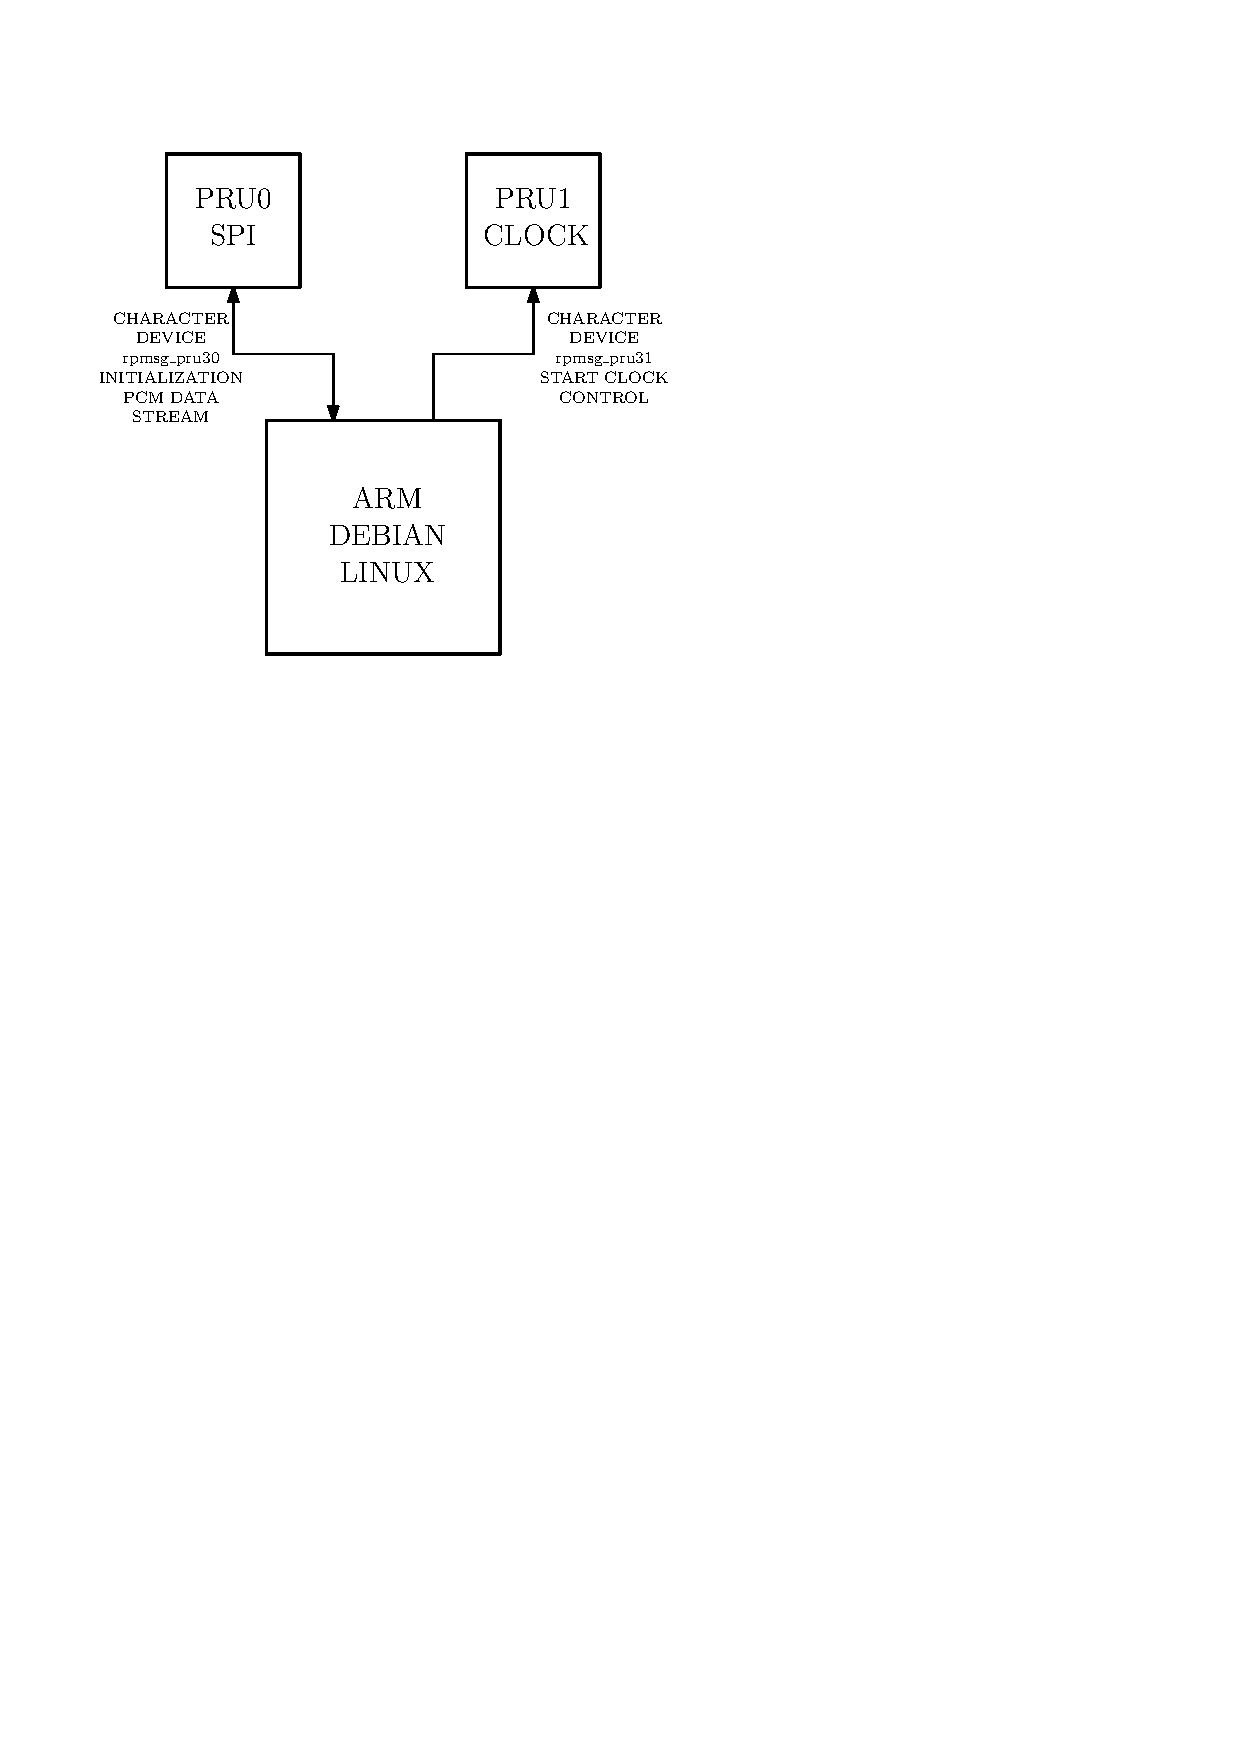
\includegraphics{diagrams/char_devices_2}
	\centering\bfseries
	\caption{PRU<->ARM Character Devices}
\end{figure}



Control of the PRU Clock Using Character Driver

